\begin{frame}{第十九讲、凹凸性与分析作图}
	\linespread{1.5}
	\begin{enumerate}
	  \item {\bf 内容与要求}{\b( \S 5.4,\S 3.3 )}
	  \begin{itemize}
	    \item 熟练掌握可导函数极值的判定方法
	    \item 掌握函数凹凸性的概念与判定方法
	    \item 掌握函数的分析作图法
% 	    \item 熟练掌握L'Hospital法则
	  \vspace{1em}
	  \end{itemize}
	  \item {\bf 课后练习:}
	  \begin{itemize}
	    \item 书面作业:{\b 习题3.3:10;习题5.4:10,12,14(3)}
%  	    \item 思考题:{\b 习题5.4:4,5,12}
	  \end{itemize}
	\end{enumerate}
\end{frame}

% \section{可导函数的极值}
% 
% \begin{frame}{函数极值的判定}
% 	\linespread{1.2}\pause 
% 	\begin{block}{{\bf 定理5.4.2}(极值第一充分条件)\hfill P265}\pause 
% 		设$f(x)$在$x_0$连续,在$x_0$的去心领域内可导,且$f\,'(x)$在$x_0$两侧导数值异号,则
% 		$f(x)$在$x_0$处取极值。\pause 
% 	\end{block}
% 	\begin{exampleblock}{{\bf 例1}\hfill }
% 		讨论以下函数的极值
% 		$$f(x)=\left(1+x+\df{x^2}{2!}+\ldots+\df{x^n}{n!}\right)e^{-x}$$
% 	\end{exampleblock}
% \end{frame}
% 
% \begin{frame}{{函数极值的判定}{\small (续)}}
% 	\linespread{1.2}\pause 
% 	\begin{block}{{\bf 定理5.4.3}(极值第二充分条件)\hfill P267}\pause 
% 		设$f(x)$在$x_0$二阶可导,且$f\,'(x_0)=0$,则
% 		\begin{enumerate}\pause 
% 		  \item 若$f\,''(x_0)<0$,$f(x)$在$x_0$处取极大值\pause 
% 		  \item 若$f\,''(x_0)>0$,$f(x)$在$x_0$处取极小值
% 		\end{enumerate}
% 	\end{block}\pause 
% 	\begin{exampleblock}{{\bf 例2}\hfill P267:例4}
% 		求函数$f(x)=x^3-6x^2+5$的极值。
% 	\end{exampleblock}
% \end{frame}
% 
% \begin{frame}
% 	\linespread{1.2}
% 	\begin{exampleblock}{{\bf 例3}\hfill P270:例7}
% 		判定方程$2^x-2x=1$有几个实根。
% 	\end{exampleblock}
% % 	\bigskip
% 	\pause 
% 	\begin{exampleblock}{{\bf 例4}\hfill P269:例8}
% 		一束光线由空气中一点$A$射入水中,经过水中一点$B$。已知光在空气和水中的
% 		传播速度分别是$v_1$和$v_2$,且光总是沿着介质中耗时最少的路径传播,
% 		试确定光线的传播路径。
% 	\end{exampleblock}
% 	\pause
% 	\begin{exampleblock}{{\bf 例5}\hfill P280:习题7}
% 		求数列$\sqrt[n]n$中最大的一项。
% 	\end{exampleblock}
% \end{frame}

\section{函数的凹凸性}

\begin{frame}{函数的凹凸性}
	\linespread{1.2}\pause
	{\bf 约定:}\alert{以下的凹凸均指“上凹”和“上凸”}\pause
	\begin{block}{{\bf 定义5.4.1}(凹函数)\hfill P273}
		设函数$f(x)$在区间$I$上有定义,若对任意$x_1,x_2\in I$,以及任意$\lambda\in[0,1]$,
		有
		$$f[\lambda x_1+(1-\lambda)x_2]\leq \lambda f(x_1)+(1-\lambda)f(x_2)$$
		则称$f(x)$是区间$I$上的{\bb 凹函数}。\pause 若上式中的等号严格成立,则称其为{\bb 严格凹函数}。
	\end{block}\pause
	{\bf 注:}\alert{任意两点间的割线都不会位于两点间曲线的下方}
\end{frame}

\begin{frame}{可导凹函数的充要条件}
	\linespread{1.2}\pause
	\begin{block}{{\bf 定理5.4.4}\hfill P275}
		设$f(x)$在$(a,b)$内可导,则$f(x)$为$(a,b)$内的凹函数,当且仅当:对任意$x_1,x_2\in(a,b)$,
		恒有
		$$f(x_2)\geq f(x_1)+f\,'(x_1)(x_2-x_1). $$
		\pause 不等号严格成立时,对应于严格凹函数的情形。
	\end{block}\pause
	{\bf 注:}\alert{任意点处的切线总位于曲线下方}
\end{frame}

\begin{frame}{凹函数的判定}
	\linespread{1.2}\pause
	\begin{block}{{\bf 定理5.4.5}(充分条件)\hfill P276}
		设$f(x)$在$(a,b)$二阶可导,则\pause
		\begin{enumerate}
		  \item 若$f\,''(x)$恒不小于零,$f(x)$为凹函数\pause
		  \item 若$f\,''(x)$恒不大于零,$f(x)$为凸函数
		\end{enumerate}
	\end{block}\pause
	{\bb 拐点:}两侧$f\,''(x)$反号的点\pause
	\begin{block}{{\bf 推论}\hfill P276:例11}
		严格凸(凹)函数的驻点为极值点。
	\end{block}
\end{frame}

\section{渐近线与分析作图法}

\begin{frame}{渐进线}
	\linespread{1}\pause
	\vspace{-1ex}
	\begin{block}{{\bf 定理3.3.5}\hfill P134}
		\begin{enumerate}\pause
		  \item {\bb 水平渐近线:}$\limx{\pm\infty}f(x)=b$\pause
		  \item {\bb 铅直渐近线:}$\limx{a^{\pm}}f(x)=\infty$\pause
		  \item {\bb 斜渐近线:}\pause
		  \begin{itemize}
		    \item 斜率:$k=\limx{\pm\infty}\df{f(x)}{x}$\pause
		    \item 截距:$b=\limx{\pm\infty}[f(x)-kx]$
		  \end{itemize}
		\end{enumerate}
	\end{block}\pause
	\vspace{-1ex}
	\begin{exampleblock}{{\bf 例6}\hfill P135:例10}
		求函数$f(x)=\df{2x^2-3}{x+1}$的渐近线。
	\end{exampleblock}
\end{frame}

\begin{frame}[t]{分析作图法}
	\linespread{1.2}\pause
	\begin{exampleblock}{{\bf 例7}\hfill P279-例14}
		作出函数$y=\df{x}{1+x^2}$的图形。
	\end{exampleblock}\pause
	
	\begin{enumerate}
	  \item {\bf 分析函数一般性质:}{\b 定义域、值域、奇偶性、周期性、与坐标轴的交点}\pause
	  \item {\bf 求一、二阶导函数:}{\b 确定不可导点}\pause
	  \item {\bf 列表分析:}{\b 单调、凸凹区间,极值点和拐点}\pause
	  \item {\bf 画出渐进线:}{\b 水平、铅直和斜渐进线}\pause
	  \item {\bf 描点作图}
	\end{enumerate}
\end{frame}

\begin{frame}[t]{分析作图法}
	\linespread{1.2}
	\begin{exampleblock}{{\bf 例8}\hfill P279-例14}
		作出函数$y=\df{x}{1+x^2}$的图形。
	\end{exampleblock}
	\begin{center}
			\resizebox{!}{5cm}{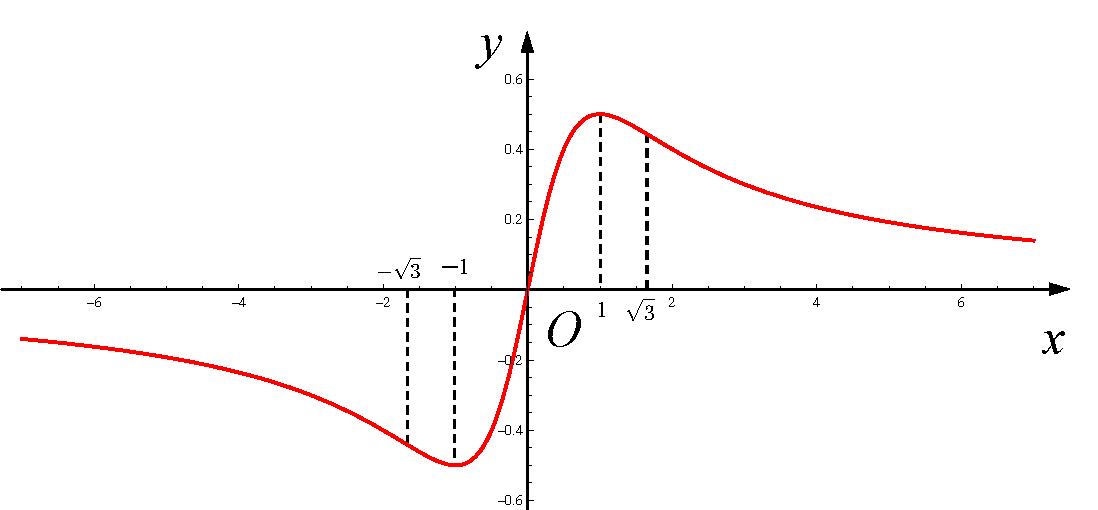
\includegraphics{./images/ch5/x1x2.pdf}}
		\end{center}
\end{frame}

\begin{frame}[<+->]{小结}
	\linespread{1.5}
	\begin{enumerate}
	  \item {\bf 可导函数的极值}
	  \item {\bf 函数的凹凸性}
	  \item {\bf 分析作图法}
	  \begin{itemize}
	    \item 定义域、值域、奇偶性、单调性、周期性、\ldots
	    \item 一、二阶导数、不可导点
	    \item 极值点、拐点、单调区间
	    \item 渐近线
	  \end{itemize}
	\end{enumerate}
% 	\bigskip
% 	\pause
% 	\centerline{\ba{请自行阅读第六章\S 6.3节}}
\end{frame}

\begin{frame}{课堂练习}
	\linespread{2}
	\begin{columns}[t]
		\column{.45\textwidth}
		\begin{exampleblock}{{\bf 例7:}函数作图}
		\centerline{\large $y=xe^{1/x}$}
		\end{exampleblock}\pause 
		\begin{itemize}
		  \item 极值点:$y(1)=e$
		  \item 渐近线:$y=x+1$
		\end{itemize}
		\pause 
		\column{.55\textwidth}
		\begin{center}
			\vspace{-3ex}
			\resizebox{!}{7cm}{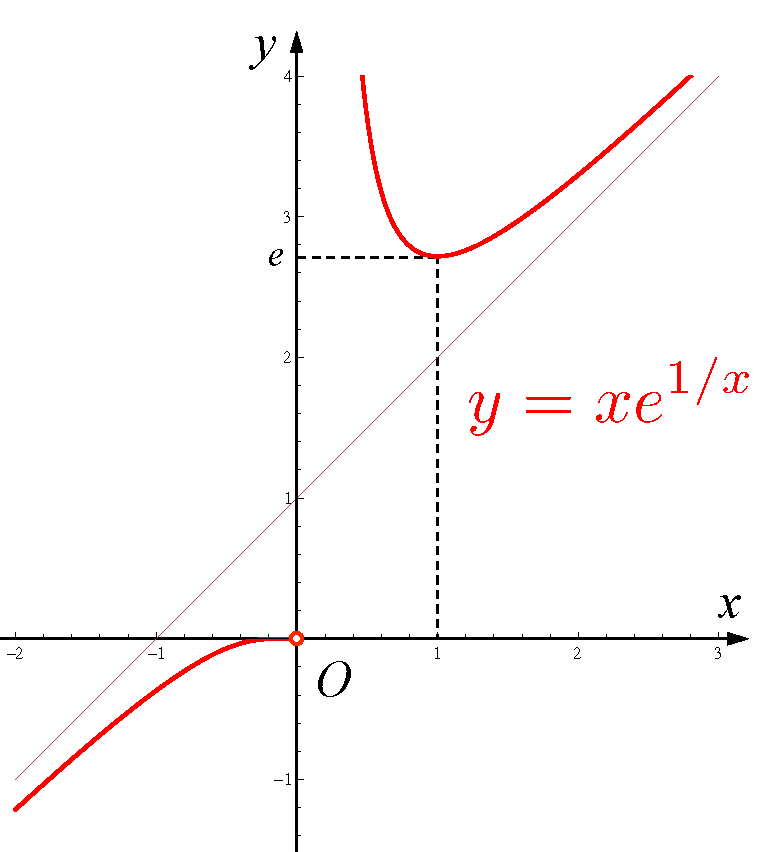
\includegraphics{./images/ch5/xe1x.pdf}}
		\end{center}
	\end{columns}
\end{frame}